\documentclass[a4paper,12pt]{ctexart} %A4纸,小四号字体
\usepackage{multirow}
\usepackage{fontspec}
\usepackage{graphicx}
\usepackage{amsmath,amssymb}
\usepackage{amsthm} % For theorem environment
\usepackage{bm}
\usepackage{xcolor}
\usepackage{listings}
\usepackage[hidelinks]{hyperref}
\usepackage{hyperref}
\usepackage{setspace}
\usepackage{booktabs}
\usepackage{caption}
\usepackage[noend]{algpseudocode}
\usepackage{algorithmicx,algorithm}
\usepackage{tikz}
\usepackage{tcolorbox}
\definecolor{learnboxback}{gray}{0.95}
\definecolor{learnboxframe}{gray}{0.75}
\newtcolorbox{learnbox}{
  colback=learnboxback,
  colframe=learnboxframe,
  title=小结
}
\newtheorem{definition}{定义}[section]
% \newtheorem{proof}{证明}[section]

% 公式编号格式设置
\makeatletter
\renewcommand{\theequation}{\arabic{section}.\arabic{equation}}
\@addtoreset{equation}{section}
\makeatother

% 设置算法环境
\floatname{algorithm}{算法}
\renewcommand{\algorithmicrequire}{\textbf{输入:}}
\renewcommand{\algorithmicensure}{\textbf{输出:}}

\newfontfamily\yaheiconsola{YaHei.Consolas.1.11b.ttf}
\setmonofont[
Contextuals={Alternate},
ItalicFont = Fira Code Retina Nerd Font Complete.otf     % to avoid font warning
]{YaHei.Consolas.1.11b.ttf}
\definecolor{codegreen}{rgb}{0,0.6,0}
\definecolor{NavyBlue}{rgb}{0.0, 0.0, 0.50}
\definecolor{PineGreen}{rgb}{0.0, 0.47, 0.44}
\lstset
{
    tabsize=4,
    captionpos=b,
    numbers=left,                    
    numbersep=1em,                  
    sensitive=true,
    showtabs=false, 
    frame=shadowbox,
    breaklines=true,
    keepspaces=true,                 
    showspaces=false,                
    showstringspaces=false,
    breakatwhitespace=false,         
    basicstyle=\yaheiconsola,
    keywordstyle=\color{NavyBlue},
    commentstyle=\color{codegreen},
    numberstyle=\color{gray},
    stringstyle=\color{PineGreen!90!black},
    rulesepcolor=\color{red!20!green!20!blue!20}
}

% 设置页面边距
\usepackage[margin=2.4cm]{geometry}
\setlength{\parindent}{2em}
\newtheorem{theorem}{Theorem} % Define theorem environment

\author{\kaishu 舒双林}
\title{\kaishu EM算法的简易教程及应用}
\date{2025年4月8日}

\begin{document}
\maketitle

\tableofcontents
\newpage

\section{EM算法的理论基础}
\setcounter{page}{1}
\begin{flushleft}
    {\kaishu EM算法是过去二十年,统计对人类科技发展的最大贡献。}
    \end{flushleft}
    \begin{flushright}
    {\kaishu —— 刘传海 教授 (美国普渡大学)}
    \end{flushright}
\subsection{什么是EM算法?}
EM算法(期望最大化算法,Expectation Maximization)是一种用于从不完全数据中估计参数的迭代方法。通过在每次迭代中交替进行期望(E步)和最大化(M步),该算法能够在给定观测数据和隐变量的条件下求解出模型的最大似然估计。

EM算法最早由Dempster等人于1977年提出,并广泛应用于统计学、机器学习等领域,尤其在缺失数据和隐变量模型中具有重要应用。
EM算法的核心思想是通过迭代地估计隐变量的期望和更新模型参数,逐步逼近最大似然估计。具体步骤为:
\begin{enumerate}
    \item E步(期望步):在当前参数估计下,计算隐变量的期望。
    \item M步(最大化步):最大化期望函数,更新参数估计值。
\end{enumerate}
通过交替进行E步和M步,EM算法逐步逼近对数似然函数的最大值。
\begin{figure}[H]
    \centering
    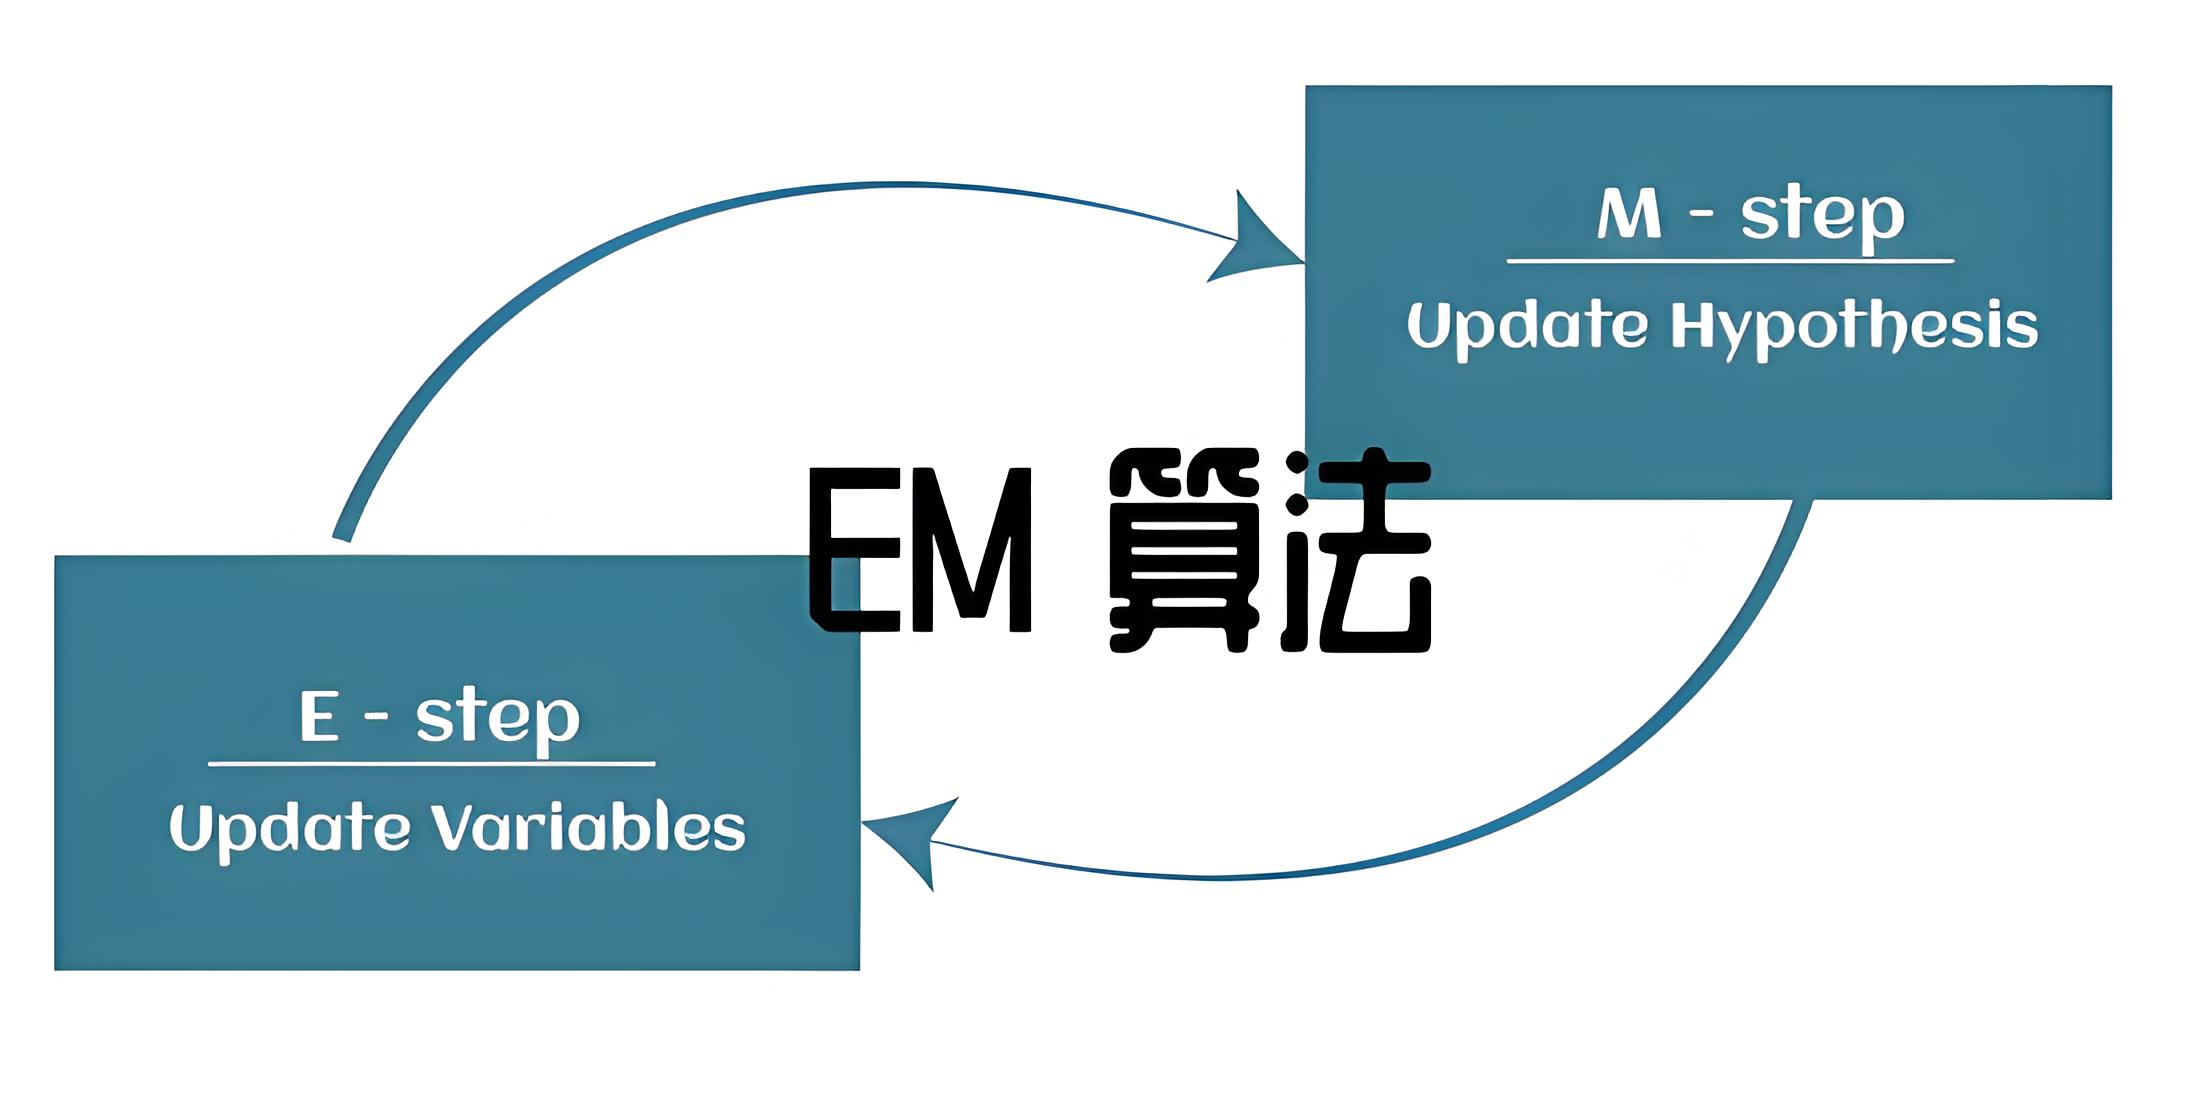
\includegraphics[width=0.7\textwidth]{fig/EM算法.jpg}
    \caption{EM算法}
    \label{fig:em_flowchart}
\end{figure}

\subsection{EM算法的数学推导}
设 \( Y \) 为观测随机变量的数据,\( Z \) 为隐变量的数据。\( Y \) 和 \( Z \) 组合起来称为完全数据,而观测数据 \( Y \) 称为不完全数据。假设给定观测数据 \( Y \),其概率分布为 \( P(Y|\theta) \),其中 \( \theta \) 是需要估计的模型参数,那么不完全数据 \( Y \) 的似然函数为 \( P(Y|\theta) \),对数似然函数为 \( L(\theta) = \log P(Y|\theta) \)。假设 \( Y \) 和 \( Z \) 的联合概率分布为 \( P(Y, Z|\theta) \),那么完全数据 \( Y \) 和 \( Z \) 的对数似然函数为:
\begin{equation}
L(\theta) = \log P(Y, Z|\theta)
\end{equation}

对于含有隐变量 \( Z \) 的概率模型,直接极大化对数似然函数 \( L(\theta) = \log P(Y|\theta) \) 是困难的,因为其含有未观测数据,并且涉及求和(或积分)的对数。

假设在第 \( i \) 次迭代后,参数的估计值为 \( \theta^{(i)} \)。考虑新的估计值 \( \theta \) 能否使 \( L(\theta) \) 增加。对 \( L(\theta) \) 和 \( L(\theta^{(i)}) \) 作差:
\begin{equation}
L(\theta) - L(\theta^{(i)}) = \log \left( \sum_{Z} P(Y|Z, \theta)P(Z|\theta) \right) - \log P(Y|\theta^{(i)})
\end{equation}
该公式表达了在不同参数下,对数似然函数的变化,用于说明参数更新的效果。

接下来,利用Jensen不等式\footnote{Jensen不等式指出,对于任意凹函数$f$和随机变量$X$,有$\mathbb{E}[f(X)] \leq f(\mathbb{E}[X])$。对于凸函数,不等号方向相反。}可得到该差值的下界:
\begin{equation}
    \begin{split}
        L(\theta) - L(\theta^{(i)}) &= \log \left( \sum_{Z} P(Z|Y, \theta^{(i)}) \frac{P(Y|Z, \theta)P(Z|\theta)}{P(Z|Y, \theta^{(i)})} \right) - \log P(Y|\theta^{(i)}) \\
&\geq \sum_{Z} P(Z|Y, \theta^{(i)}) \log \frac{P(Y|Z, \theta)P(Z|\theta)}{P(Z|Y, \theta^{(i)})} - \log P(Y|\theta^{(i)}) \\
&= \sum_{Z} P(Z|Y,\theta^{(i)}) \log \frac{P(Y|Z,\theta)P(Z|\theta)}{P(Z|Y,\theta^{(i)})P(Y|\theta^{(i)})}
    \end{split}
\end{equation}
令
\begin{equation}
    B(\theta,\theta^{(i)}) = L(\theta^{(i)}) + \sum_{Z} P(Z|Y,\theta^{(i)}) \log \dfrac{P(Y|Z,\theta)P(Z|\theta)}{P(Z|Y,\theta^{(i)})P(Y|\theta^{(i)})} 
    \label{eq1}
\end{equation}
则

\[
L(\theta) \geq B(\theta, \theta^{(i)}) 
\]
即函数 \( B(\theta, \theta^{(n)}) \) 是 \( L(\theta) \) 的一个下界,而且由式\eqref{eq1}可知:

\begin{equation}
L(\theta^{(i)}) = B(\theta^{(i)}, \theta^{(i)})
\end{equation}


因此,任何可以使 \( B(\theta, \theta^{(i)}) \) 增大的 \(\theta\),也可以使 \( L(\theta) \) 增大。为了使 \( L(\theta) \) 有尽可能大的增长,选择 \(\theta^{(i+1)}\) 使 \( B(\theta, \theta^{(i)}) \) 达到极大,即

\begin{equation}
    \theta^{(n+1)} = \arg \max_{\theta} B(\theta, \theta^{(n)})
    \label{eq2}
\end{equation}

\begin{definition}[Q函数]

    设 \( P(Y, Z|\theta) \) 为观测数据和隐变量的联合分布,\( P(Z|Y, \theta^{(i)}) \) 为在给定观测数据 \( Y \) 和当前参数估计 \( \theta^{(i)} \) 下隐变量 \( Z \) 的条件概率分布,则定义函数 \( Q(\theta, \theta^{(i)}) \) 为:
    \begin{equation}
        Q(\theta, \theta^{(i)}) = \sum_{Z} P(Z|Y, \theta^{(i)}) \log P(Y, Z|\theta)
    \end{equation}
    
\end{definition}

此处定义的 \( Q(\theta, \theta^{(i)}) \) 函数是EM算法的核心,为EM算法中E步和M步的关键。
可以证明,最大化 \( Q(\theta, \theta^{(i)}) \) 将确保 \( L(\theta) \) 不减。因此,EM算法的迭代公式为:
\begin{equation}
\theta^{(i+1)} = \arg \max_{\theta} Q(\theta, \theta^{(i)})
\end{equation}
\begin{proof}
    若去掉 \(\theta\) 的极大化而言是常数的项,由式\eqref{eq2}和式\eqref{eq1},有
\begin{equation}
    \begin{split}
        \theta^{(i+1)} &= \arg \max_{\theta} \left( L(\theta^{(i)}) + \sum_{Z} P(Z|Y, \theta^{(i)}) \log \frac{P(Y|Z, \theta)P(Z|\theta)}{P(Z|Y, \theta^{(i)})P(Y|\theta^{(i)})} \right) \\
        &= \arg \max_{\theta} \left( \sum_{Z} P(Z|Y, \theta^{(i)}) \log(P(Y|Z, \theta)P(Z|\theta)) \right) \\
        &= \arg \max_{\theta} \left( \sum_{Z} P(Z|Y, \theta^{(i)}) \log P(Y, Z|\theta) \right) \\
        &= \arg \max_{\theta} Q(\theta, \theta^{(i)})
    \end{split}
    \label{eq3}
\end{equation}
\end{proof}

式\eqref{eq3}等价于 EM 算法的一次迭代,即求 \( Q \) 函数及其极大化。EM 算法是通过不断求解下界的极大化逼近求解对数似然函数极大化的算法。


上述推导包含了EM算法的两个主要步骤:

\begin{enumerate}
    \item E步:计算 \( Q(\theta, \theta^{(i)}) \)
    \item M步:求解 \( \theta^{(i+1)} = \arg \max_{\theta} Q(\theta, \theta^{(i)}) \)
\end{enumerate}

通过不断求解下界的极大化,EM算法逐步逼近对数似然函数的极大值,但无法保证找到全局最优解。
\begin{figure}[H]
    \centering
    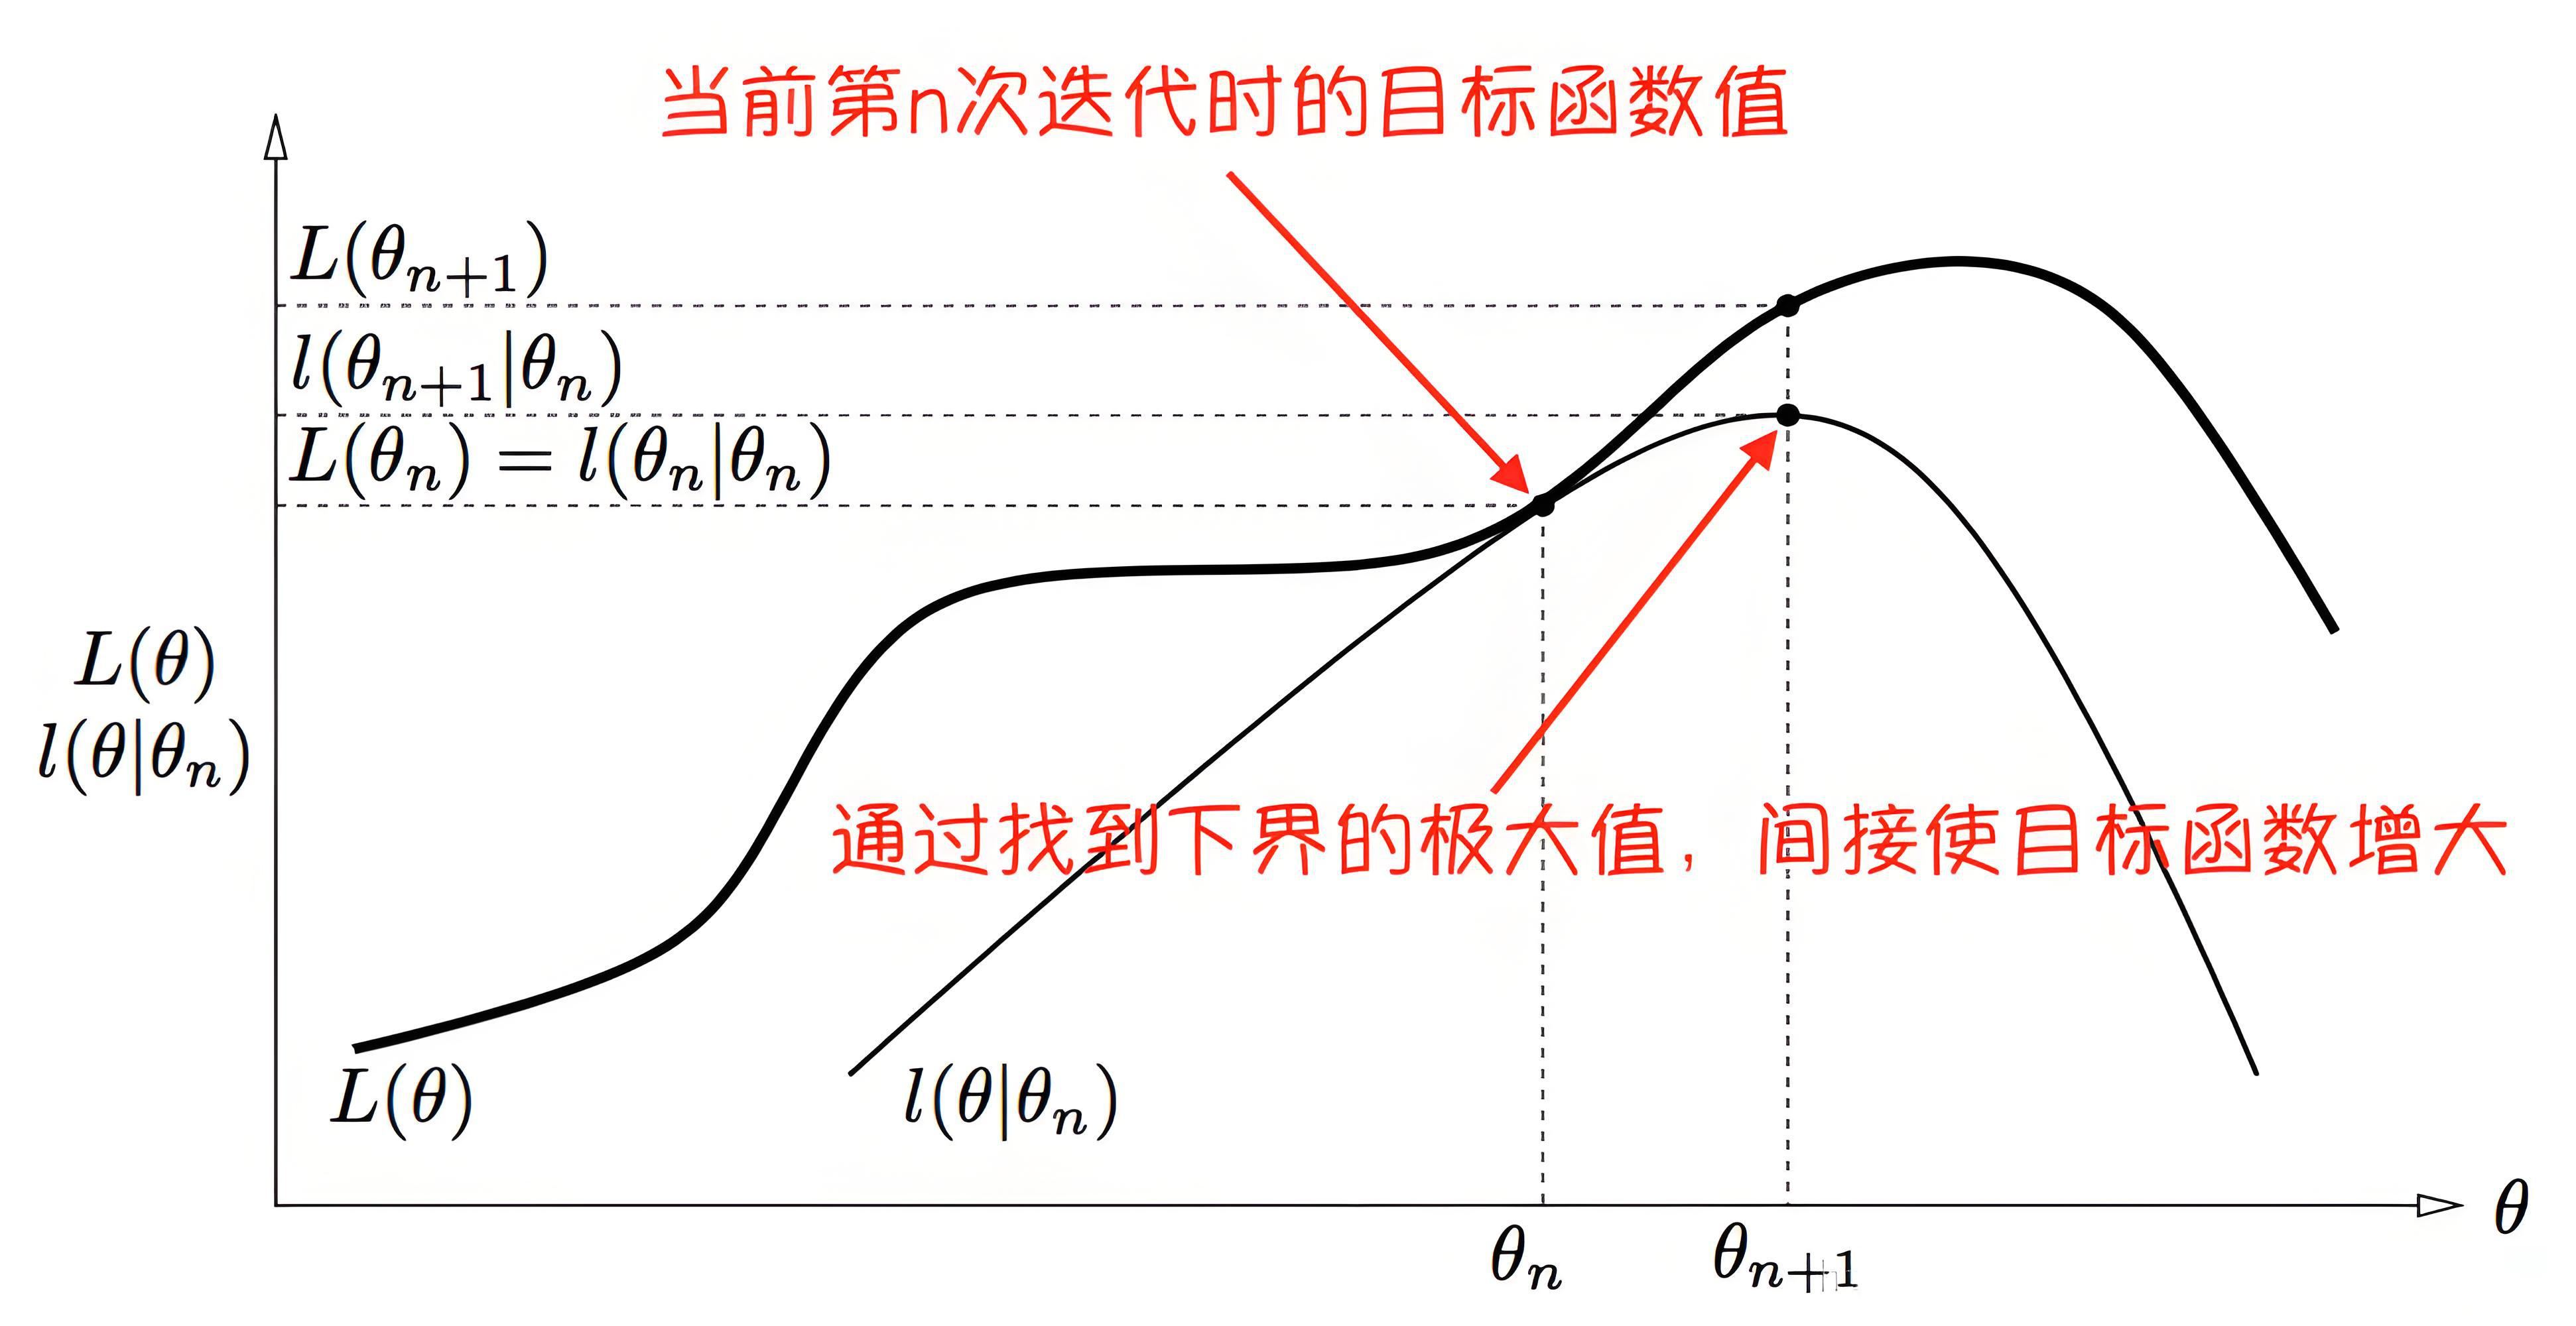
\includegraphics[width=0.9\textwidth]{fig/EM算法示意图.jpg}
    \caption{EM算法示意图}
\end{figure}
\subsection{EM算法的收敛性}

EM算法的收敛性是通过以下定理来保证的:

\begin{theorem}[单调性]
设 \( P(Y|\theta) \) 为观测数据的似然函数,\( \theta^{(i)} \)(\( i = 1, 2, \dots \))为EM算法得到的参数估计序列,则 \( P(Y|\theta^{(i)}) \) 是单调递增的,即:
\begin{equation}
P(Y|\theta^{(i+1)}) \geq P(Y|\theta^{(i)})
\end{equation}
\end{theorem}

\begin{proof}
    令
    \begin{equation}
    H(\theta, \theta^{(i)}) = \sum_Z \log P(Z | Y, \theta) P(Z | Y, \theta^{(i)})
    \label{eq:H_definition}
    \end{equation}
    
    于是对数似然函数可以写成
    \begin{equation}
    \log P(Y | \theta) = Q(\theta, \theta^{(i)}) - H(\theta, \theta^{(i)})
    \label{eq:log_likelihood}
    \end{equation}
    
    在式 \eqref{eq:log_likelihood} 中分别取 $\theta$ 为 $\theta^{(i)}$ 和 $\theta^{(i+1)}$ 并相减,有
    \begin{equation}
    \log P(Y | \theta^{(i+1)}) - \log P(Y | \theta^{(i)}) 
    = \left[ Q(\theta^{(i+1)}, \theta^{(i)}) - Q(\theta^{(i)}, \theta^{(i)}) \right] 
    - \left[ H(\theta^{(i+1)}, \theta^{(i)}) - H(\theta^{(i)}, \theta^{(i)}) \right]
    \label{eq:log_diff}
    \end{equation}
    
    为证式 \eqref{eq:log_diff},只需证式右端是非负的。式 \eqref{eq:log_diff} 右端的第 1 项,由于 $\theta^{(i+1)}$ 使得 $Q(\theta, \theta^{(i)})$ 达到极大,所以有
    \begin{equation}
    Q(\theta^{(i+1)}, \theta^{(i)}) - Q(\theta^{(i)}, \theta^{(i)}) \geq 0
    \label{eq:Q_nonnegative}
    \end{equation}
    
    其第 2 项,由式 \eqref{eq:H_definition} 可得:
    \begin{equation}
    H(\theta^{(i+1)}, \theta^{(i)}) - H(\theta^{(i)}, \theta^{(i)}) 
    = \sum_Z \left( \log \frac{P(Z | Y, \theta^{(i+1)})}{P(Z | Y, \theta^{(i)})} \right) P(Z | Y, \theta^{(i)})
    \label{eq:H_diff}
    \end{equation}
    
    由 Jensen 不等式,有
    \begin{equation}
    \sum_Z \left( \log \frac{P(Z | Y, \theta^{(i+1)})}{P(Z | Y, \theta^{(i)})} \right) P(Z | Y, \theta^{(i)})
    \leq \log \left( \sum_Z \frac{P(Z | Y, \theta^{(i+1)})}{P(Z | Y, \theta^{(i)})} P(Z | Y, \theta^{(i)}) \right)
    \label{eq:Jensen}
    \end{equation}
    
    因此
    \begin{equation}
    H(\theta^{(i+1)}, \theta^{(i)}) - H(\theta^{(i)}, \theta^{(i)}) 
    \leq \log \left( \sum_Z P(Z | Y, \theta^{(i+1)}) \right) = 0
    \label{eq:H_diff_final}
    \end{equation}
    
    由式 \eqref{eq:Q_nonnegative} 和式 \eqref{eq:H_diff_final} 即知式 \eqref{eq:log_diff} 右端是非负的。
    
\end{proof}

\begin{theorem}[收敛性]
设 \( L(\theta) = \log P(Y|\theta) \) 为观测数据的对数似然函数,\( \theta^{(i)} \)(\( i = 1, 2, \dots \))为EM算法得到的参数估计序列,\( L(\theta^{(i)}) \)(\( i = 1, 2, \dots \))为对应的对数似然函数序列。则:
\begin{enumerate}
    \item 收敛性:如果 \( P(Y|\theta) \) 有上界,则 \( L(\theta^{(i)}) \) 收敛到某一值 \( L^* \)。
    \item 稳定点性质:在函数 \( Q(\theta, \theta') \) 与 \( L(\theta) \) 满足一定条件下,由EM算法得到的参数估计序列 \( \theta^{(i)} \) 的收敛值 \( \theta^* \) 是 \( L(\theta) \) 的稳定点。
\end{enumerate}
\end{theorem}

\begin{proof}
    (1) 由 $L(\theta) = \log P(Y | \theta^{(i)})$ 的单调性及 $P(Y | \theta)$ 的有界性立即得到。
    
    (2) 设 $L(\theta)$ 的极大值点为 $\theta^*$,则有
    \begin{equation}
    \begin{aligned}
    L(\theta^{(i)}) - L(\theta^*) &= Q(\theta^{(i)}, \theta^*) - H(\theta^{(i)}, \theta^*) 
    \leq Q(\theta^{(i)}, \theta^{(i)}) - H(\theta^{(i)}, \theta^*) \\
    &\leq Q(\theta^{(i)}, \theta^{(i)}) - H(\theta^{(i)}, \theta^{(i)}) 
    = L(\theta^{(i)}) - L(\theta^{(i)}) = 0
    \end{aligned}
    \end{equation}
    由此可知,$L(\theta^{(i)})$ 收敛到 $L(\theta^*)$,即 $\theta^{(i)}$ 收敛到 $\theta^*$。
    由于 $L(\theta)$ 的极大值点是唯一的,所以 $\theta^*$ 是 $L(\theta)$ 的稳定点。

    \end{proof}

\subsection{EM算法流程}

\begin{center}
    \begin{minipage}{0.95\textwidth}
        \begin{algorithm}[H]
            \caption{EM算法} 
            \label{alg:em}
            {\bf 输入:} 观测变量数据Y、隐变量数据Z、联合分布$P(Y,Z|\theta)$、条件分布$P(Z|Y,\theta)$\\
            {\bf 过程:} 
            \begin{algorithmic}[1]
                \State 选择参数初值$\theta^{(0)}$、最大迭代次数N、迭代精度$\delta$,开始迭代
                \For{$i = 1$ to $N$}
                \State 令$\theta^{(i-1)}$为第$i-1$次迭代参数$\theta$的估计值
                \State E-step:计算在给定观测数据Y和当前参数$\theta^{(i-1)}$下Z的条件概率分布期望
                \begin{equation}
                        Q(\theta,\theta^{(i-1)}) = \sum_Z\log P(Y,Z|\theta)P(Z|Y,\theta^{(i-1)})
                \end{equation}
                \State M-step:极大化$Q(\theta,\theta^{(i-1)})$,确定第$i$次迭代的参数估计值$\theta^{(i)}$
                \begin{equation}
                    \theta^{(i)} = \arg \max_{\theta}Q(\theta,\theta^{(i-1)})
                \end{equation}
                \State 计算$\theta^{(i-1)}$与$\theta^{(i)}$的差值的二范数$\delta^{(i)}=||\theta^{(i)}-\theta^{(i-1)}||$
                \If{$\delta^{(i)}$ < $\delta$}
                \State 迭代结束,$\hat{\theta} = \theta^{(i)}$为参数的极大似然估计值
                \Else
                \State 继续迭代,$i = i + 1$,返回第3步
                \EndIf
                \EndFor
                \State 迭代结束,$\hat{\theta} = \theta^{(N)}$为参数的极大似然估计值
            \end{algorithmic}
            {\bf 输出:} 模型的参数估计值$\hat{\theta}$
        \end{algorithm}
    \end{minipage}
\end{center}

关于EM算法的实施过程,需要注意以下几点:
\begin{enumerate}
    \item 参数的初值选择可以任意,但需注意EM算法对初值敏感性较高,不同的初值可能导致不同的收敛结果。
    \item 迭代停止的条件可以基于参数变化或$Q$函数增益,即:
    \begin{equation}
    \|\theta^{(i+1)} - \theta^{(i)}\| < \delta_1 \quad \text{或} \quad \|Q(\theta^{(i+1)},\theta^{(i)}) - Q(\theta^{(i)},\theta^{(i)})\| < \delta_2
    \end{equation}
    \item M步求解$Q(\theta,\theta^{(i)})$的极大化,得到$\theta^{(i+1)}$,完成一次迭代$\theta^{(i)} \to \theta^{(i+1)}$。前述的单调性和收敛性定理保证了EM算法的收敛性。
\end{enumerate}

\subsection{EM算法的应用场景}

EM算法的优势在于能够有效地从不完全数据中估计参数,且实现相对简单。该算法被广泛应用于统计学、机器学习、数据挖掘等领域,尤其在处理缺失数据和隐变量模型时具有重要作用。常见的应用场景包括:
\begin{itemize}
    \item 高斯混合模型(GMM):对多模态数据进行建模和聚类
    \item 隐马尔可夫模型(HMM):时序数据分析与模式识别
    \item 潜在语义分析(LSA):文本挖掘与主题建模
    \item 概率主成分分析(PPCA):降维与特征提取
\end{itemize}

这些应用场景共同点在于均存在隐变量或缺失数据,需要通过迭代方法进行参数估计。

\section{EM算法的应用}

EM算法广泛应用于统计学、机器学习以及数据科学等领域,尤其在缺失数据、隐变量模型、聚类分析等问题中展现了其强大的能力。以下将介绍EM算法在几个经典应用中的具体实现与分析。

\subsection{硬币问题}

\subsubsection{问题描述}
假设有两枚不规则硬币A和B,硬币A正面出现的概率为$p$,硬币B正面出现的概率为$q$。随机选择其中一枚硬币,并投掷10次,共进行5轮,记录如下数据,其中"H"表示正面,"T"表示反面。任务是估计硬币A和硬币B正面出现的概率$p$和$q$。

\begin{table}[H]
    \centering
    \caption{硬币投掷结果}
    \begin{tabular}{ccccccccccccc}
    \toprule
     & coin & 1 & 2 & 3 & 4 & 5 & 6 & 7 & 8 & 9 & 10 & result \\
    \midrule
    1 & ? & H & T & T & T & H & H & T & H & T & H & 5H5T \\
    2 & ? & H & H & H & H & T & H & H & H & H & H & 9H1T \\
    3 & ? & H & T & H & H & H & H & H & T & H & H & 8H2T \\
    4 & ? & H & T & H & T & T & T & H & H & T & T & 4H6T \\
    5 & ? & T & H & H & H & T & H & H & H & T & H & 7H3T \\
    \bottomrule
    \end{tabular}
\end{table}

\subsubsection{EM算法求解硬币问题}
为了估计硬币A和B的正面概率$p$和$q$,应用EM算法进行求解。EM算法通过交替进行E步和M步来估计这两个参数。

在E步,根据当前参数估计,计算出每轮投掷中选择硬币A或硬币B的概率。M步则基于E步计算得到的概率,更新硬币A和硬币B的正面概率$p$和$q$。

通过不断迭代E步和M步,最终得到收敛的参数估计值。

EM算法的具体步骤如下:
\begin{enumerate}
    \item 初始化参数$p^{(0)} = 0.6, q^{(0)} = 0.5$
    \item E步:
    \begin{itemize}
        \item 计算隐变量的期望
        \begin{align*}
            p_1^{(1)} &= P(Z_1=A|X,p^{(0)},q^{(0)}) = \frac{p^{5}(1-p)^5}{p^5(1-p)^{5} + q^{5}(1-q)^5}  \approx 0.4491 \\
            q_1^{(1)} &= P(Z_1=B|X,p^{(0)},q^{(0)}) = 1-  P(Z_1=A|X,p^{(0)},q^{(0)})\approx 0.5509 \\
            \vdots \nonumber \\
            p_5^{(1)} &= P(Z_5=A|X,p^{(0)},q^{(0)}) =\frac{p^{7}(1-p)^3}{p^7(1-p)^{3} + q^{7}(1-q)^3} \approx 0.6472 \\
            q_5^{(1)} &= P(Z_5=B|X,p^{(0)},q^{(0)}) = 1-  P(Z_5=A|X,p^{(0)},q^{(0)})\approx 0.3528 
        \end{align*}

        \item 计算A、B硬币的正反面次数的期望并更新参数
        \begin{align*}
        E^{(1)}_A(H) &= p_1^{(1)} \times 5 + p_2^{(1)} \times 9 + \cdots + p_5^{(1)} \times 7 = 21.2975 \\
        E^{(1)}_A(T) &= p_1^{(1)} \times 5 + p_2^{(1)} \times 1 + \cdots + p_5^{(1)} \times 3 = 8.5722 \\
        E^{(1)}_B(H) &= q_1^{(1)} \times 5 + q_2^{(1)} \times 9 + \cdots + q_5^{(1)} \times 7 = 11.7025\\
        E^{(1)}_B(T) &= q_1^{(1)} \times 5 + q_2^{(1)} \times 1 + \cdots + q_5^{(1)} \times 3 = 8.4278 
        \end{align*}
    \end{itemize}
    
    \item M步:计算参数的极大似然估计
    \begin{align*}
    p^{(1)} &= \frac{E^{(1)}_A(H)}{E^{(1)}_A(H) + E^{(1)}_A(T)} = \frac{21.2975}{21.2975+8.5722} \approx 0.7130 \\
    q^{(1)} &= \frac{E^{(1)}_B(H)}{E^{(1)}_B(H) + E^{(1)}_B(T)} = \frac{11.7025}{11.7025+8.4278} \approx 0.5813 
    \end{align*}

    \item 重复E步和M步,直到收敛,最终得到结果:
    \begin{equation*}
    \hat{p} = p^{(11)} = 0.7968, \hat{q} = q^{(11)} = 0.5196
    \end{equation*}
\end{enumerate}

\subsubsection{结果分析}
通过EM算法的迭代过程,最终获得了硬币A和硬币B正面出现的概率估计。最终的结果为:
\begin{equation*}
    \hat{p} = p^{(11)} = 0.7968, \hat{q} = q^{(11)} = 0.5196
\end{equation*}

\begin{table}[htbp]
    \centering
    \caption{EM算法迭代过程(收敛阈值$\delta=10^{-4}$)}
    \begin{tabular}{p{2cm}p{2cm}p{2cm}p{2cm}p{2cm}}
    \toprule
    \textbf{迭代次数} & \textbf{$p$值} & \textbf{$\Delta p$} & \textbf{$q$值} & \textbf{$\Delta q$} \\
    \midrule
    0 & 0.6000 & -- & 0.5000 & -- \\
    1 & 0.7130 & 0.1130 & 0.5813 & 0.0813 \\
    2 & 0.7453 & 0.0323 & 0.5693 & -0.0120 \\
    $\vdots$ & $\vdots$ & $\vdots$ & $\vdots$ & $\vdots$ \\
    10 & 0.7967 & 0.0001 & 0.5197 & -0.0001 \\
    11 & 0.7968 & 0.0000 & 0.5196 & -0.0000 \\
    \bottomrule
    \end{tabular}
\end{table}
这些结果表明,硬币A的正面概率较高,而硬币B的正面概率较低。随着迭代次数的增加,参数估计逐渐收敛,EM算法成功地从不完全的投掷数据中估计出硬币的正面概率。这表明EM算法在处理缺失数据和隐变量问题时能够高效且准确地给出估计值。

本案例的源代码见附录\ref{sec:coin_code}。

\subsection{桦尺蛾问题}

\subsubsection{背景介绍}
桦尺蛾是一个典型的自然选择和工业污染的进化案例。这些蛾子的颜色由一个基因决定,存在三个可能的等位基因:C、I 和 T。C是显性基因,T是隐性基因,而I是对C显性、对T隐性的基因。桦尺蛾的表现型包括:

\begin{itemize}
    \item \textbf{Carbonaria型}:具有纯黑的颜色(由CC、CI和CT基因型表现)。
    \item \textbf{Typica型}:具有浅色的有图案的翅膀(由TT基因型表现)。
    \item \textbf{Insularia型}:颜色中等,通常表现为斑驳的中等色(由II和IT基因型表现)。
\end{itemize}

\begin{figure}[htbp]
    \centering
    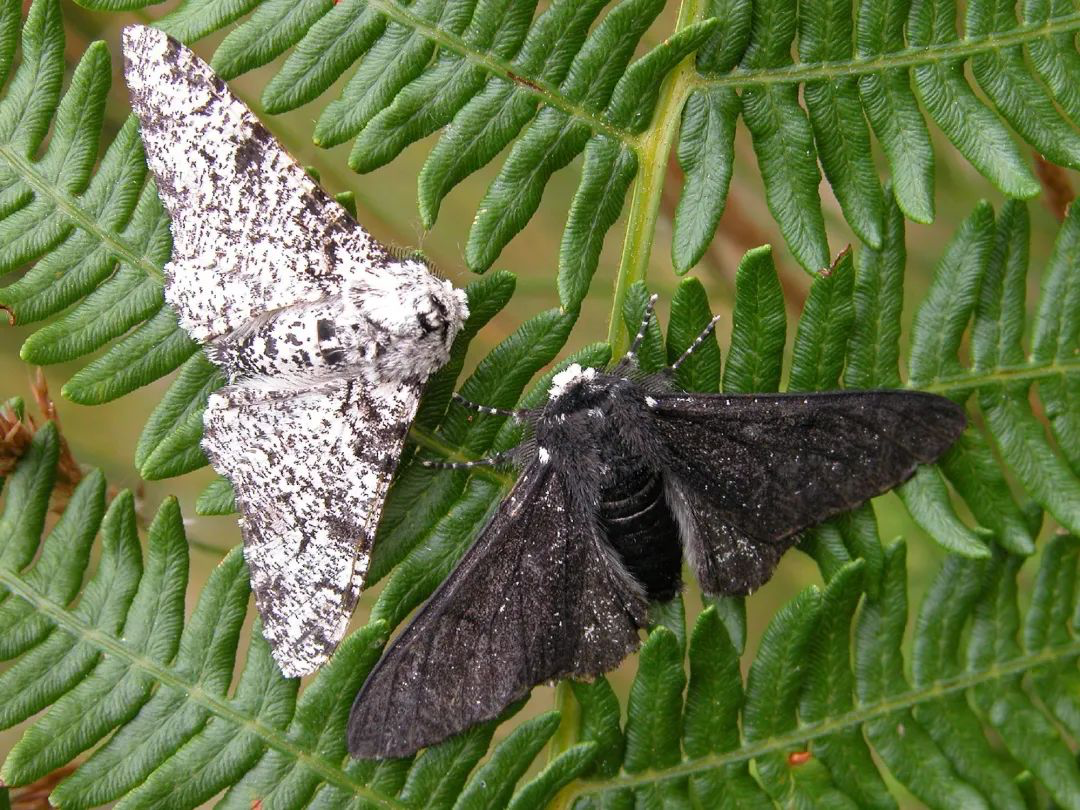
\includegraphics[width=0.6\textwidth]{fig/桦尺蛾.png}
    \caption{桦尺蛾的不同表现型}
    \label{fig:moths}
\end{figure}

由于环境污染的影响,Carbonaria型蛾子数量显著增加,因此需要估计三种等位基因C、I和T的频率,进而理解基因型的变化。

\subsubsection{EM算法估计基因频率}
桦尺蛾有六种可能的基因型,但现场调查中只能够测量三种表现型。
\begin{itemize}
    \item \textbf{基因型CC、CI、CT}:表现为Carbonaria表现型(黑色)
    \item \textbf{基因型II、IT}:表现为Insularia表现型(中等颜色,斑驳)
    \item \textbf{基因型TT}:表现为Typica表现型(浅色)
\end{itemize}

为了从仅有的表现型数据中估计等位基因频率,需要应用EM算法。其中E步计算在已知表现型数据的情况下,各基因型的期望计数,而M步则根据E步的期望更新基因频率。

\textbf{EM算法步骤}:
\begin{enumerate}
    \item 初始化等位基因频率
    \begin{itemize}
        \item 假设初始等位基因频率为 $p_C^{(0)}$、$p_I^{(0)}$、$p_T^{(0)}$,满足 $p_C^{(0)} + p_I^{(0)} + p_T^{(0)} = 1$。
    \end{itemize}
    
    \item E步
    \begin{itemize}
        \item 在已知表现型数据的情况下,估计每种基因型的期望计数。
        \item 对于碳化表现型(carbonaria),可能的基因型为 $CC$、$CI$、$CT$。计算每种基因型的概率:
        \begin{align*}
            P(CC | \text{carbonaria}) &= \frac{p_C^2}{p_C^2 + 2p_Cp_I + 2p_Cp_T} \\
            P(CI | \text{carbonaria}) &= \frac{2p_Cp_I}{p_C^2 + 2p_Cp_I + 2p_Cp_T} \\
            P(CT | \text{carbonaria}) &= \frac{2p_Cp_T}{p_C^2 + 2p_Cp_I + 2p_Cp_T}
        \end{align*}
        \item 使用概率计算期望基因型计数(其他基因型类似):      
        \begin{align*}
        n_{CC}^{(t)} &= n_C \cdot P(CC | \text{carbonaria}) \\
        n_{CI}^{(t)} &= n_C \cdot P(CI | \text{carbonaria}) \\
        n_{CT}^{(t)} &= n_C \cdot P(CT | \text{carbonaria})
        \end{align*}
    \end{itemize}
    
    \item M步: 使用E步得到的期望基因型计数,更新等位基因频率:
        \begin{align*}
        p_C^{(t+1)} &= \frac{2n_{CC}^{(t)} + n_{CI}^{(t)} + n_{CT}^{(t)}}{2n} \\
        p_I^{(t+1)} &= \frac{2n_{II}^{(t)} + n_{CI}^{(t)} + n_{IT}^{(t)}}{2n} \\
        p_T^{(t+1)} &= \frac{2n_{TT}^{(t)} + n_{CT}^{(t)} + n_{IT}^{(t)}}{2n}
        \end{align*}
    
    \item 迭代: 重复E步和M步,直到等位基因频率收敛。
\end{enumerate}

\subsubsection{结果分析}
经过多次迭代,EM算法成功估计出三种等位基因的频率,最终结果为:
\begin{equation*}
p_C = 0.4, \quad p_I = 0.3, \quad p_T = 0.3
\end{equation*}

\begin{figure}[H]
    \centering
    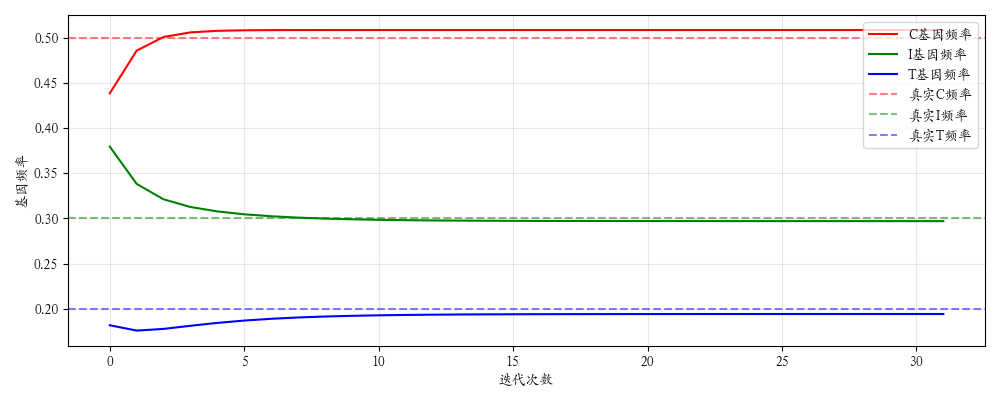
\includegraphics[width=0.72\textwidth]{fig/蛾迭代.png}
    \caption{等位基因频率迭代收敛过程}
    \label{fig:moth_iteration}
\end{figure}

这些结果表明,基因C的频率最高,I和T的频率相对较低。这些信息有助于解释桦尺蛾的表现型在不同环境条件下的变化,并为后续的生物学研究提供了依据。

详细实现代码请参见\ref{sec:peppered_moths_code}。
\subsection{高斯混合模型}

高斯混合模型(Gaussian Mixture Model, GMM)是一种常用的聚类方法,具有如下形式的概率分布形式:
\begin{equation}
P(y|\theta) = \sum_{k=1}^K \alpha_k \phi(y|\theta_k)
\end{equation}
其中,$\alpha_k$为混合系数,$\phi(y|\theta_k)$为高斯分布密度函数,$\theta_k = (\mu_k,\sigma_k^2)$为高斯分布的均值和方差,
\begin{equation}
\phi(y|\theta_k) = \frac{1}{\sqrt{2\pi}\sigma_k} \exp\left(-\frac{(y-\mu_k)^2}{2\sigma_k^2}\right)
\end{equation}
称为第$k$个高斯分布的密度函数。

\subsubsection{EM算法在高斯混合模型中的应用}
EM算法在GMM中的应用非常广泛,通过迭代更新高斯分布的参数(均值、方差和混合系数),从而对数据进行建模。

假设有一组数据$y_1,y_2,\cdots,y_n$,服从高斯混合模型,即
\begin{equation}
P(y|\theta) = \sum_{k=1}^K \alpha_k \phi(y|\theta_k)
\end{equation}
其中,$\theta = \{\alpha_k,\mu_k,\sigma_k^2\}_{k=1}^K$为模型参数。EM算法估计高斯混合模型的参数的步骤如下:

\begin{enumerate}
    \item 初始化参数$\theta^{(0)} = \{\alpha_k^{(0)},\mu_k^{(0)},\sigma_k^{2(0)}\}_{k=1}^K$,计算对数似然函数$L(\theta^{(0)})$。
    
    \item E步:对于每个数据点$y_i$,计算其属于第$k$个高斯分量的后验概率
    \begin{equation}
    \gamma_{ik} = \frac{\alpha_k^{(t)}\phi(y_i|\theta_k^{(t)})}{\sum_{j=1}^K \alpha_j^{(t)}\phi(y_i|\theta_j^{(t)})}
    \end{equation}
    
    \item M步:基于E步计算的后验概率更新参数估计
    \begin{align}
    \alpha_k^{(t+1)} &= \frac{1}{n} \sum_{i=1}^n \gamma_{ik} \\
    \mu_k^{(t+1)} &= \frac{\sum_{i=1}^n \gamma_{ik}y_i}{\sum_{i=1}^n \gamma_{ik}} \\
    \sigma_k^{2(t+1)} &= \frac{\sum_{i=1}^n \gamma_{ik}(y_i-\mu_k^{(t+1)})^2}{\sum_{i=1}^n \gamma_{ik}}
    \end{align}
    
    \item 计算对数似然函数
    \begin{equation}
    L(\theta^{(t+1)}) = \sum_{i=1}^n\log\left(\sum_{k=1}^K \alpha_k^{(t+1)}\phi(y_i|\theta_k^{(t+1)})\right)
    \end{equation}
    
    \item 检查收敛条件:$|L(\theta^{(t+1)}) - L(\theta^{(t)})| < \epsilon$,若满足则停止迭代,否则继续从E步开始下一轮迭代。
\end{enumerate}

\subsubsection{高斯混合模型案例}
\begin{flushleft}
    \textbf{1.参数设置}
\end{flushleft}

本案例使用如下参数设置:
\begin{itemize}
    \item 真实混合系数:$\alpha = [0.3, 0.4, 0.3]$
    \item 真实均值:$\mu = [-2.0, 0.0, 4.0]$
    \item 真实标准差:$\sigma = [0.5, 0.8, 1.5]$
    \item 样本数量:$n = 1000$
\end{itemize}
\begin{figure}[H]
    \centering
    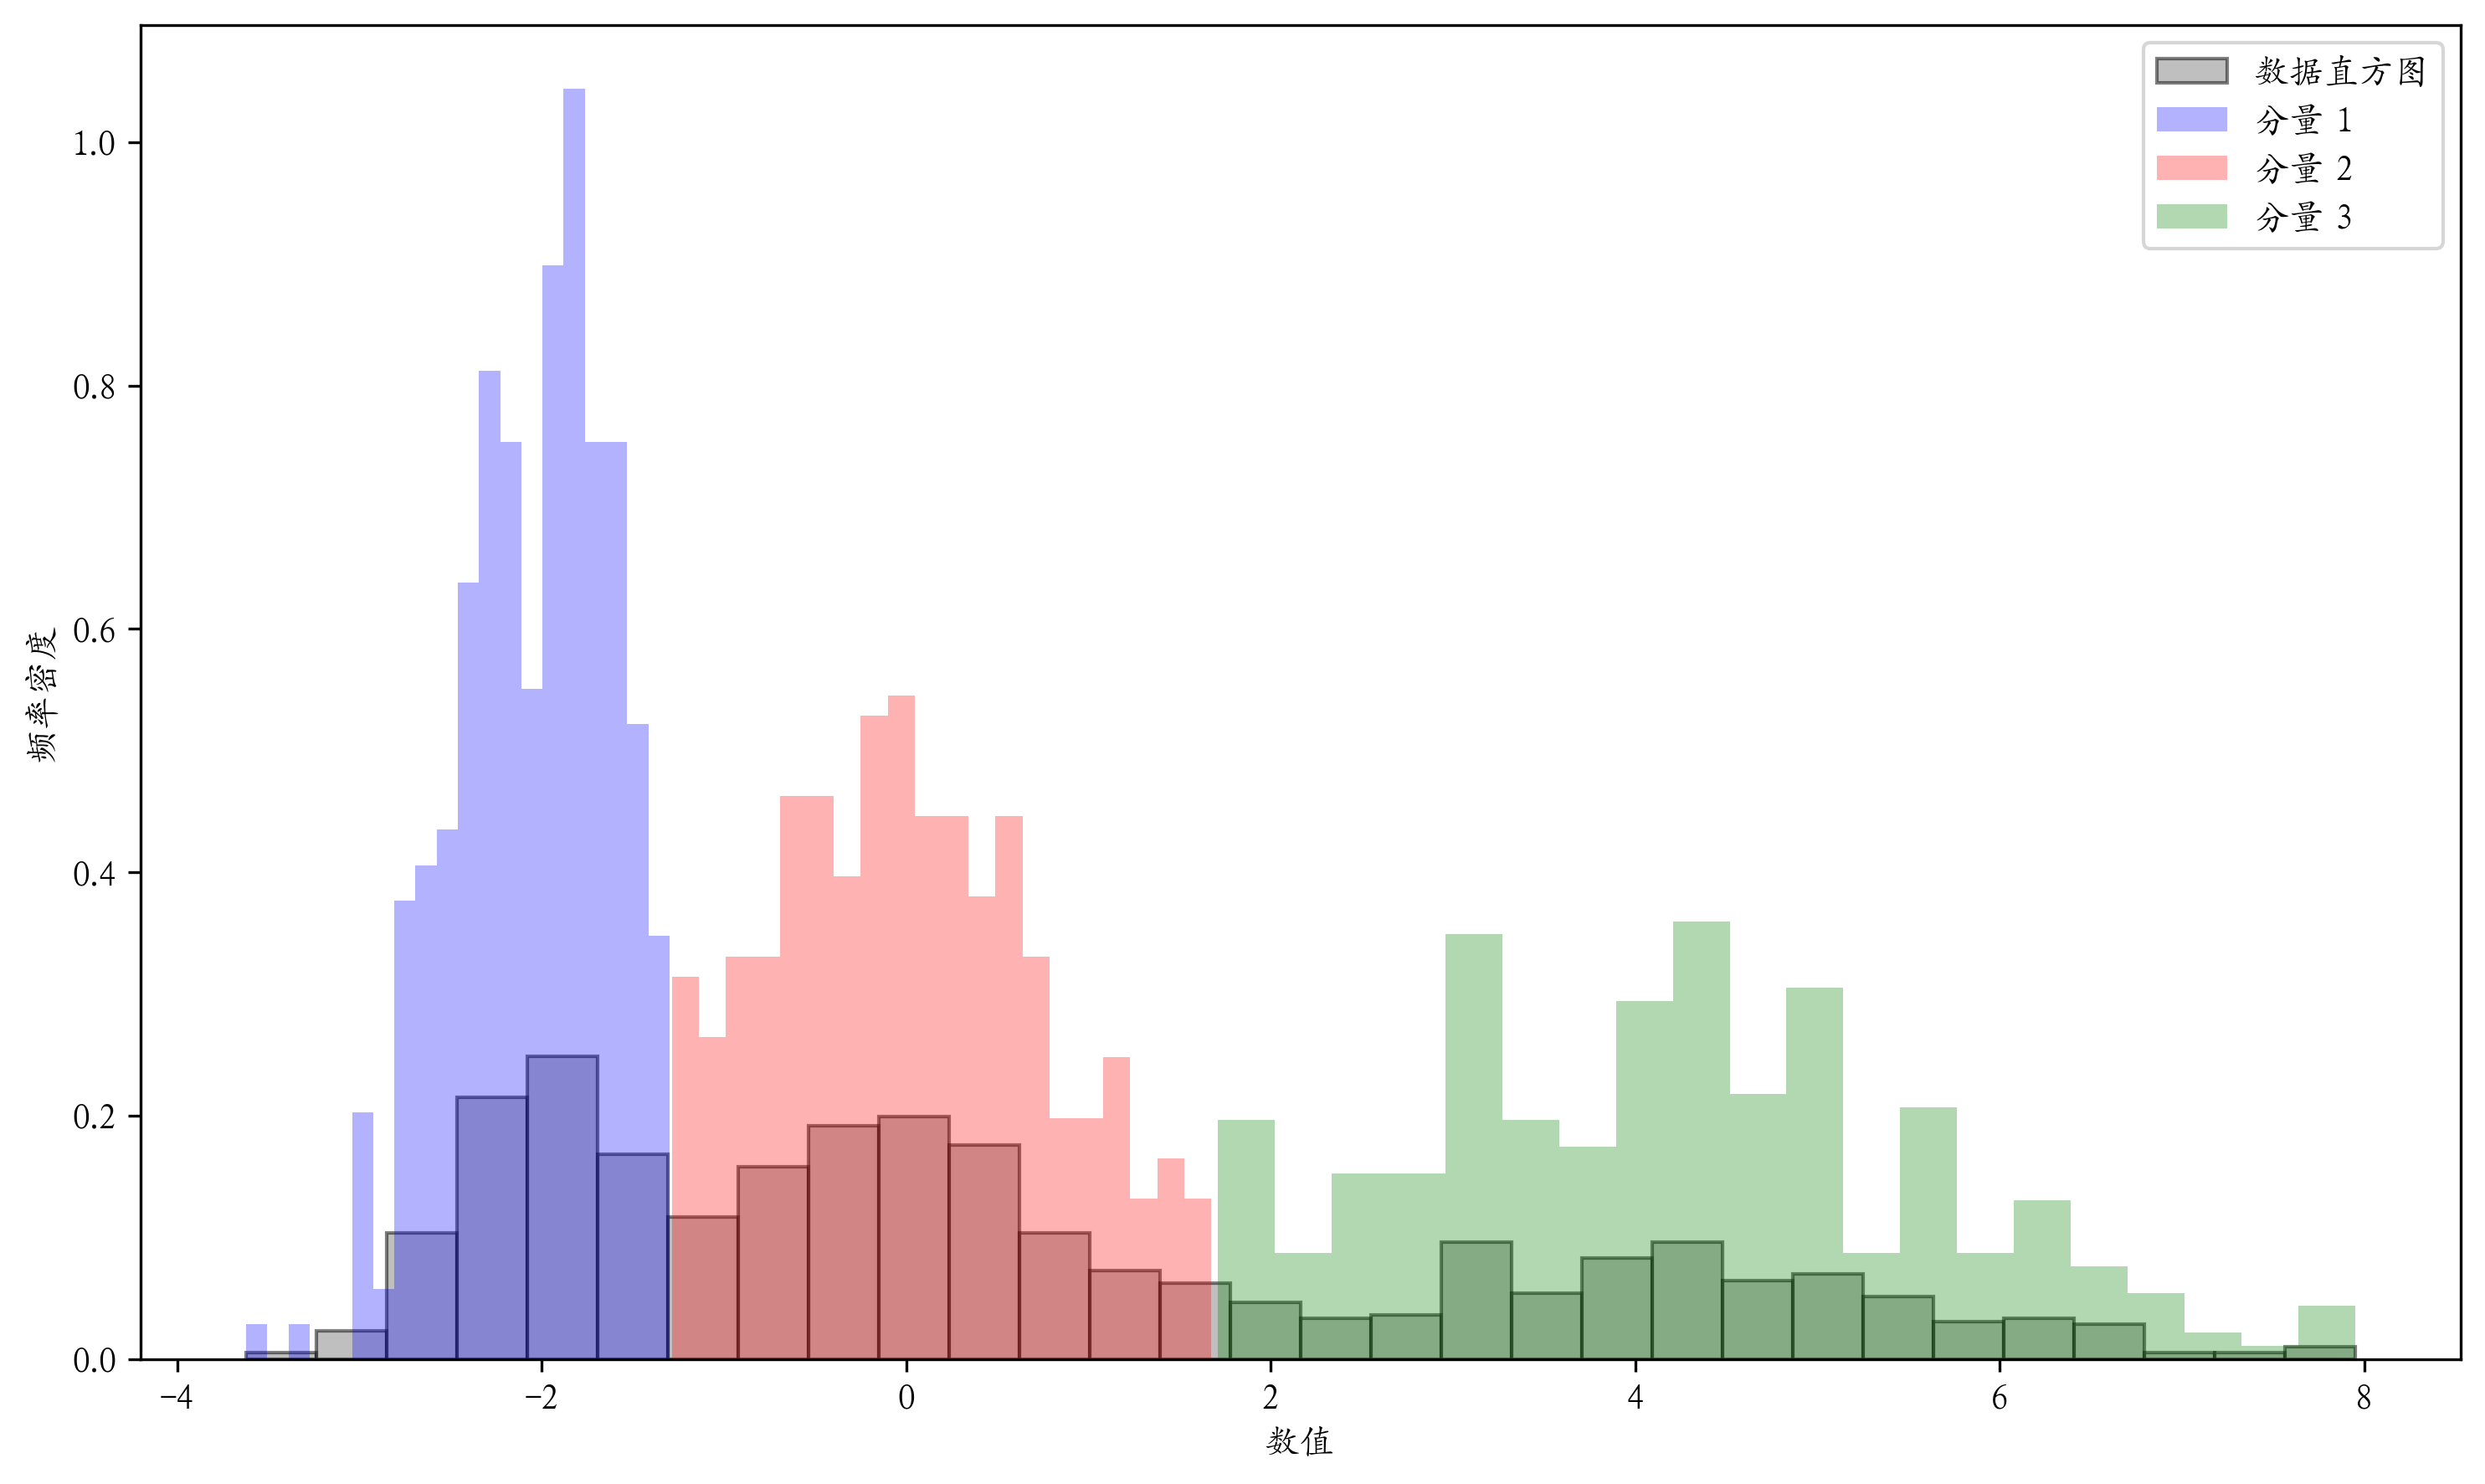
\includegraphics[width=0.7\textwidth]{fig/gmm_histogram.png}
    \caption{数据分布与成分分解}
    \label{fig:gmm_histogram}
\end{figure}

根据上述参数生成数据,数据分布如图(\ref{fig:gmm_histogram})所示。可以看到,数据呈现出三个高斯分布的混合特征。

\begin{flushleft}
    \textbf{2.EM算法实现步骤}
\end{flushleft}

EM算法通过迭代方式估计模型参数,包括以下步骤:

\begin{enumerate}
    \item \textbf{数据生成}:根据指定的混合系数、均值和标准差生成$n=1000$个样本点
    
    \item \textbf{参数初始化}:
    \begin{itemize}
        \item 混合系数$\alpha_k^{(0)} = 1/K$(初始时设每个组分权重相等)
        \item 均值$\mu_k^{(0)}$在数据范围内均匀分布,确保初始均值能够覆盖整个数据空间
        \item 标准差$\sigma_k^{(0)}$基于数据的整体标准差设定
    \end{itemize}
    
    \item \textbf{E步(期望步)}:对每个数据点$y_i$,计算其属于第$k$个高斯组分的后验概率(责任度)
    \begin{equation*}
    \gamma_{ik} = \frac{\alpha_k^{(t)}\phi(y_i|\mu_k^{(t)}, \sigma_k^{2(t)})}{\sum_{j=1}^K \alpha_j^{(t)}\phi(y_i|\mu_j^{(t)}, \sigma_j^{2(t)})}
    \end{equation*}
    
    \item \textbf{M步(最大化步)}:基于E步计算的后验概率更新参数估计
    \begin{align*}
    \alpha_k^{(t+1)} &= \frac{1}{n} \sum_{i=1}^n \gamma_{ik} \\
    \mu_k^{(t+1)} &= \frac{\sum_{i=1}^n \gamma_{ik}y_i}{\sum_{i=1}^n \gamma_{ik}} \\
    \sigma_k^{2(t+1)} &= \frac{\sum_{i=1}^n \gamma_{ik}(y_i-\mu_k^{(t+1)})^2}{\sum_{i=1}^n \gamma_{ik}}
    \end{align*}
    
    \item \textbf{计算对数似然}:评估模型拟合质量并检查收敛情况
    \begin{equation*}
    L(\theta^{(t+1)}) = \sum_{i=1}^n\log\left(\sum_{k=1}^K \alpha_k^{(t+1)}\phi(y_i|\theta_k^{(t+1)})\right)
    \end{equation*}
    
    \item \textbf{收敛判断}:检查参数变化或对数似然函数变化是否小于预设阈值
    \begin{itemize}
        \item 参数变化:$\|\theta^{(t+1)} - \theta^{(t)}\| < \epsilon_1$
        \item 对数似然变化:$|L(\theta^{(t+1)}) - L(\theta^{(t)})| < \epsilon_2$
    \end{itemize}
    
    \item \textbf{重复迭代}:如未收敛,返回第3步继续迭代,直到满足收敛条件或达到最大迭代次数
\end{enumerate}

\subsubsection{结果分析与评估}

经过多轮迭代,EM算法成功估计出三个高斯分布的参数。最终估计结果与真实值的比较如下:
\begin{table}[H]
    \centering
    \caption{EM算法多模型参数估计对比}
    \begin{tabular}{l *{9}{c}}
    \toprule
    \multirow{2}{*}{参数} & 
    \multicolumn{3}{c}{模型1} & 
    \multicolumn{3}{c}{模型2} & 
    \multicolumn{3}{c}{模型3} \\
    \cmidrule(lr){2-4} \cmidrule(lr){5-7} \cmidrule(lr){8-10}
     & 真实值 & 估计值 & 误差 & 真实值 & 估计值 & 误差 & 真实值 & 估计值 & 误差 \\
    \midrule
    $\alpha$ & 
    0.30 & 0.28 & \textcolor{red}{-0.02} & 
    0.40 & 0.41 & \textcolor{red}{0.01} & 
    0.30 & 0.30 & \textcolor{red}{0.00} \\
    
    $\mu$ & 
    -2.00 & -2.04 & \textcolor{red}{-0.04} & 
    0.00 & -0.06 & \textcolor{red}{-0.06} & 
    4.00 & 4.09 & \textcolor{red}{0.09} \\
    
    $\sigma$ & 
    0.50 & 0.46 & \textcolor{red}{-0.04} & 
    0.80 & 0.84 & \textcolor{red}{0.04} & 
    1.50 & 1.48 & \textcolor{red}{-0.02} \\
    \bottomrule
    \end{tabular}
\end{table}

观察结果可以得出以下分析:
\begin{itemize}
    \item 所有参数估计都非常接近真实值,表明EM算法在本案例中取得了良好的拟合效果
    \item 混合系数($\alpha$)的估计尤为准确,三个组分的误差均在0.02以内
    \item 均值参数($\mu$)的估计较为精确,最大偏差仅为0.09(第三组分)
    \item 标准差($\sigma$)的估计也很准确,最大偏差为0.04(第一和第二组分)
\end{itemize}

\begin{figure}[htbp]
    \centering
    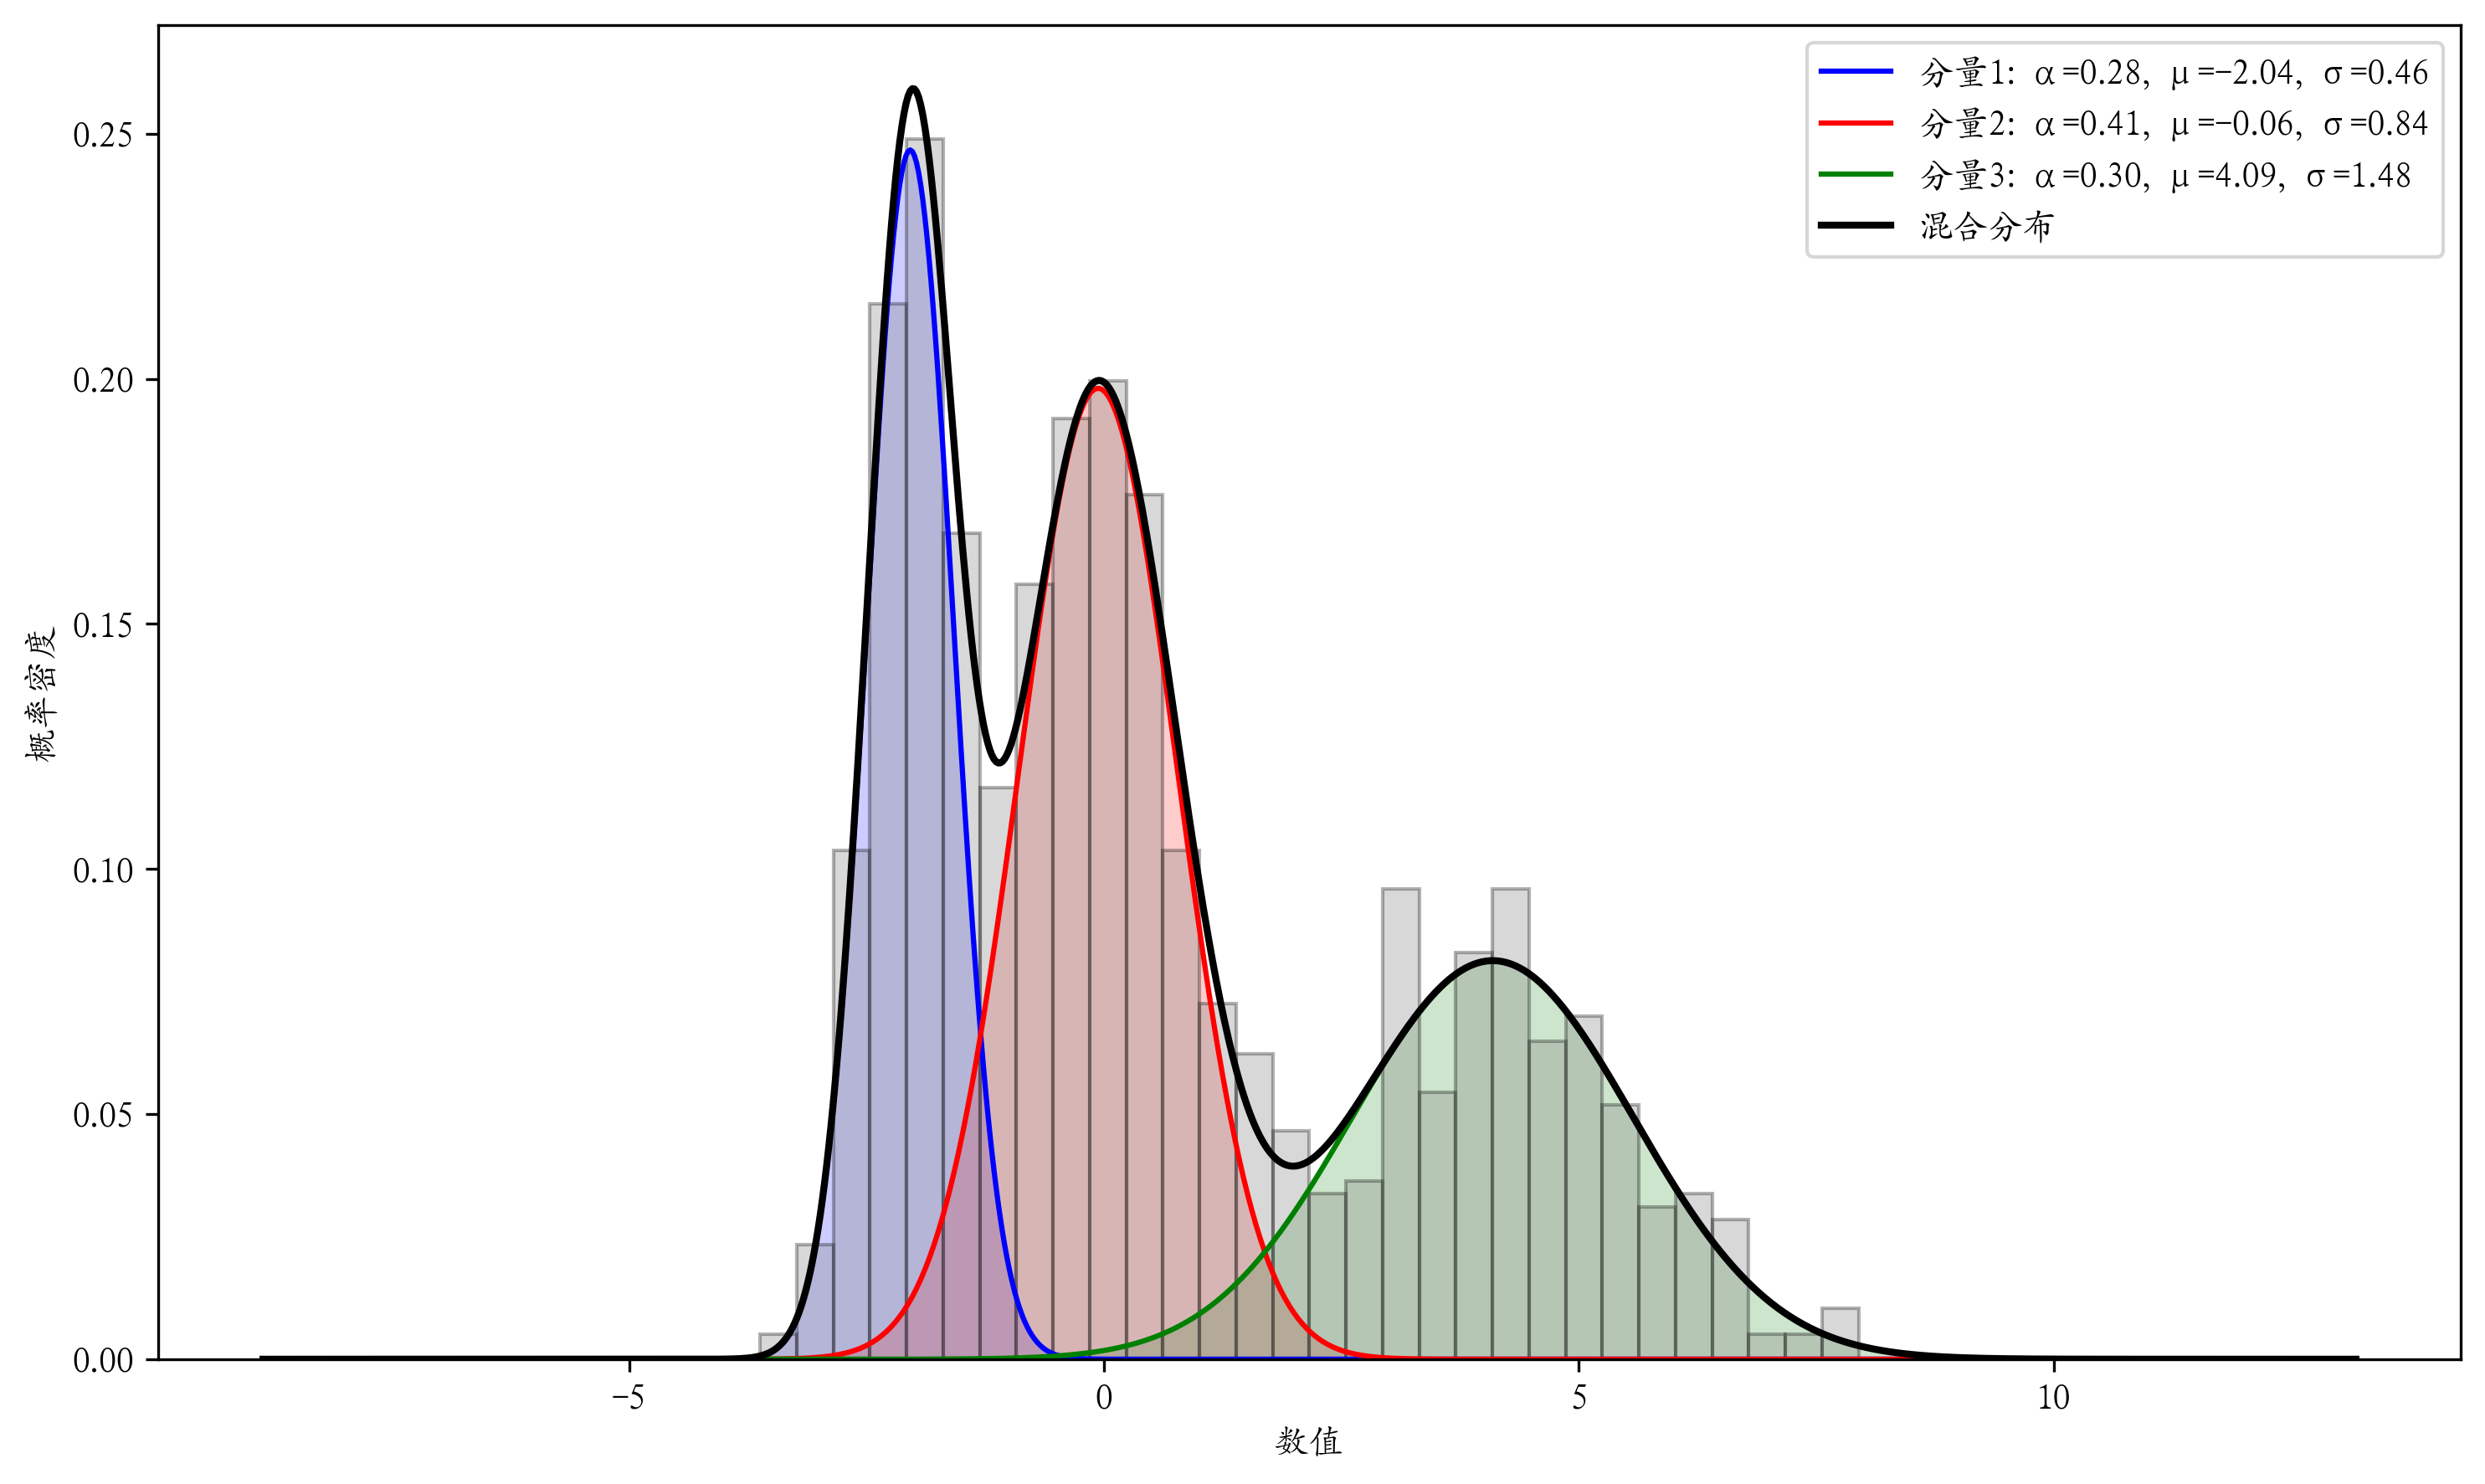
\includegraphics[width=0.7\textwidth]{fig/gmm_density.png}
    \caption{估计的高斯混合模型概率密度 - 黑线为混合分布,彩色曲线为各组分分布}
    \label{fig:gmm_density}
\end{figure}

最终,EM算法成功地对多模态数据进行了建模,识别出数据中的三个高斯分布组分。每个数据点被分配到最可能的高斯分量,这对数据聚类和密度估计具有重要意义。这种软聚类方法比K-means等硬聚类方法提供了更丰富的概率信息,能够更好地描述数据的内在结构。

通过可视化混合分布及其组分分布(如图\ref{fig:gmm_density}所示),我们可以直观地理解数据的多模态性质及EM算法的拟合效果。该案例充分展示了EM算法在处理含隐变量的复杂模型中的有效性和实用价值。

有关GMM的完整代码实现请参见附录\ref{sec:gmm_code}。

\subsection{应用总结}

EM算法在实际应用中的效果非常显著,尤其是在处理不完全数据和隐变量模型时,能够提供准确且高效的参数估计。在硬币问题、桦尺蛾问题和高斯混合模型等应用中,EM算法都展示了其强大的适应性和实用性。通过不断交替进行E步和M步,EM算法可以逐步逼近最大似然估计,在许多领域中得到广泛应用。

\begin{learnbox}{\kaishu
EM算法通过期望(E步)和最大化(M步)交替进行,能够有效处理隐变量模型和缺失数据。通过实际应用案例,如硬币问题、桦尺蛾问题和高斯混合模型,EM算法展示了其在实际问题中的强大能力,尤其是在多模态数据建模和基因频率估计等方面。}
\end{learnbox}

\section{EM算法的推广:GEM算法}

\subsection{GEM算法的背景与动机}

EM算法(期望最大化)在处理含有隐变量的最大似然估计问题时有着广泛应用,但在一些实际问题中,标准的EM算法在M步的求解上存在一定困难,尤其当$Q$函数无法通过解析方法直接求解时。这时,GEM算法(Generalized EM Algorithm)应运而生,作为EM算法的一种推广形式,它通过放宽对M步的要求,允许在M步中仅要求$Q$函数增大,而不必求解其极大值。

标准EM算法要求M步找到使期望函数$Q(\theta, \theta^{(i)})$最大化的参数$\theta^{(i+1)}$,即:
\begin{equation}
\theta^{(i+1)} = \arg \max_{\theta} Q(\theta, \theta^{(i)})
\end{equation}
而在GEM算法中,M步不要求$Q$函数的最大化,只需要找到一个使$Q$增大的$\theta^{(i+1)}$,即:
\begin{equation}
Q(\theta^{(i+1)}, \theta^{(i)}) \geq Q(\theta^{(i)}, \theta^{(i)})
\end{equation}
这使得GEM算法具有更大的灵活性,可以在许多复杂的高维问题中应用,尤其是在$Q$函数无法解析最大化时。

\subsection{GEM算法的工作原理}

GEM算法与EM算法的最大区别在于M步的处理方式。具体来说,EM算法要求M步通过优化$Q$函数来找到参数的极大似然估计,而GEM算法允许在M步中通过数值方法,找到一个能够增加$Q$函数的解,而不需要追求极大化。

\begin{itemize}
    \item \textbf{E步:} 与EM算法相同,计算隐变量$Z$的后验分布,并计算$Q(\theta, \theta^{(i)})$,该函数表示在当前参数估计下对数似然的期望。
    \item \textbf{M步:} 不要求找到使$Q$最大化的参数,而是找到一个使得$Q$函数增大的解。这使得M步不再是严格的最优化问题,可以采用数值优化技术进行近似求解。
\end{itemize}

这种修改使得GEM算法能够灵活地处理一些复杂的、不能直接求解$Q$函数最大值的问题。与EM算法相比,GEM算法具有更强的适应性,尤其在解决高维度问题时,它能避免陷入求解$Q$函数最大值的困难。

\subsection{GEM算法的迭代过程}

GEM算法的迭代过程遵循EM算法的基本框架,但放宽了M步的最大化要求。其主要步骤如下:

\begin{enumerate}
    \item \textbf{E步(期望步):} 给定当前的参数估计值$\theta^{(i)}$,计算隐变量$Z$的后验分布,并计算辅助函数$Q(\theta, \theta^{(i)})$,该函数表示对数似然函数在当前估计下的期望。
    \begin{equation}
    Q(\theta, \theta^{(i)}) = \mathbb{E}_{Z|Y, \theta^{(i)}} [\log P(Y, Z | \theta)]
    \end{equation}
    
    \item \textbf{M步(最大化步):} 不要求$Q(\theta, \theta^{(i)})$达到最大值,而是寻找一个$\theta^{(i+1)}$,使得$Q(\theta, \theta^{(i)})$增大,即:
    \begin{equation}
    Q(\theta^{(i+1)}, \theta^{(i)}) \geq Q(\theta^{(i)}, \theta^{(i)})
    \end{equation}
    这一过程可以通过数值优化方法来实现,而不一定要求解析解。
    
    \item \textbf{收敛判断:} 在每一轮迭代中,计算参数变化是否小于预设的阈值$\delta$,或者$Q$函数的增量是否足够小:
    \begin{equation}
    \|\theta^{(i+1)} - \theta^{(i)}\| < \delta
    \quad \text{或} \quad
    |Q(\theta^{(i+1)}, \theta^{(i)}) - Q(\theta^{(i)}, \theta^{(i)})| < \delta_2
    \end{equation}
    当满足这些条件时,算法结束。
\end{enumerate}

\subsection{GEM算法的优势与局限性}

\subsubsection{优势}
\begin{itemize}
    \item \textbf{灵活性:} GEM算法通过放宽M步的最大化要求,使其在一些无法通过解析方法求解$Q$函数最大值的情况下,仍能进行有效的参数估计。
    \item \textbf{适应复杂问题:} 当模型复杂,无法直接求解$Q$的极大值时,GEM算法能够通过数值优化方法,灵活地处理这些问题。
    \item \textbf{提高计算效率:} 在某些问题中,求解$Q$的最大值是非常计算密集型的,GEM算法可以通过采用梯度下降等数值方法来近似求解,从而提高计算效率。
\end{itemize}

\subsubsection{局限性}
\begin{itemize}
    \item \textbf{收敛速度较慢:} 由于GEM算法不要求严格最大化$Q$函数,其收敛速度通常比EM算法慢,尤其是在没有显式最优化的情况下。
    \item \textbf{依赖数值优化方法:} GEM算法通常需要使用数值优化方法,这可能会增加计算的复杂性,并且在某些高维度问题中可能会变得计算密集。
    \item \textbf{容易陷入局部最优:} 由于GEM算法只要求$Q$增大,而不是极大化,可能导致算法仅收敛到局部最优解。
\end{itemize}

\subsection{GEM算法的应用场景}

GEM算法的灵活性使其在多个领域中得到了应用,特别是在无法解析求解的高维复杂模型中。以下是GEM算法的典型应用场景:

\begin{itemize}
    \item \textbf{高斯混合模型 (GMM):} GEM算法用于高斯混合模型中的参数估计,尤其在模型的复杂度较高,无法解析求解$Q$函数时,使用数值方法进行近似优化。
    \item \textbf{隐马尔可夫模型 (HMM):} 在HMM中,当模型的转移概率或观测概率无法通过解析方法求解时,GEM算法提供了有效的解决方案。
    \item \textbf{主题模型:} 在自然语言处理领域,特别是LDA(Latent Dirichlet Allocation)模型中,GEM算法可以用于估计潜在主题的分布。
    \item \textbf{贝叶斯推断:} 在一些复杂的贝叶斯推断问题中,GEM算法通过数值优化方法估计后验分布,尤其适用于高维度和复杂的模型。
\end{itemize}

\subsection{GEM算法小结}

GEM算法作为EM算法的扩展,放宽了M步的优化要求,使得它在许多复杂的统计模型中具有重要应用。通过只要求$Q$函数增大而不是极大化,GEM算法在高维问题和难以解析的模型中表现出色。然而,这种放宽条件也导致了其收敛速度较慢,且可能依赖数值优化方法。

\begin{learnbox}{\kaishu
GEM算法通过放宽EM算法M步的最大化要求,使其在处理高维度、复杂模型时更加灵活。虽然它的收敛速度较慢,且可能依赖数值优化方法,但它在许多应用中表现出了强大的适应性,特别是在隐马尔可夫模型、主题模型等复杂问题中,提供了一种有效的解决方案。}
\end{learnbox}

\section{总结}

本文详细介绍了EM算法及其应用,并探讨了其在各种实际问题中的有效性和局限性。EM算法是一种处理含隐变量问题的经典方法,广泛应用于统计学、机器学习和数据科学领域。通过本文的探讨,可以清晰地了解到EM算法的理论框架、应用流程、以及不同场景下的具体应用。以下是本文的主要总结内容:

\subsection{EM算法的理论体系}

EM算法的核心思想是通过交替进行期望步(E步)和最大化步(M步)来逐步逼近最大似然估计。在E步,EM算法估计隐变量的期望,而在M步则通过最大化期望函数来更新模型参数。通过这种交替的迭代过程,EM算法能够有效处理含有隐变量的统计模型。

本文详细推导了EM算法的数学基础,使用了Jensen不等式来求得对数似然函数的下界,并通过最大化辅助函数$Q(\theta, \theta^{(i)})$来更新参数。此外,EM算法具有良好的收敛性,可以保证似然函数单调递增,但无法保证达到全局最优解,这也是EM算法的一大局限性。

\subsection{EM算法的应用与反思}

EM算法在多个实际问题中取得了显著成果。通过硬币问题、桦尺蛾基因频率估计以及高斯混合模型的应用,展示了EM算法在处理不完全数据和隐变量模型时的强大能力。在硬币问题中,EM算法通过迭代计算隐变量的期望并更新参数估计,成功估计出了硬币正面出现的概率。在桦尺蛾基因频率估计中,EM算法通过观测到的表现型数据推断了基因型的分布,为生物学研究提供了理论依据。而在高斯混合模型中,EM算法则用于估计混合高斯分布的参数,从而对多模态数据进行建模。

然而,EM算法也有其局限性。首先,EM算法对初始值较为敏感,可能导致算法陷入局部最优解。其次,在处理高维数据时,EM算法的计算效率可能成为瓶颈,尤其是在M步的最大化计算中,需要耗费大量的计算资源。未来的研究方向应关注如何提高EM算法的计算效率,并减少对初值的依赖。

\subsection{EM算法的拓展与未来发展}

随着计算技术的不断进步,EM算法在许多实际问题中的应用得到不断扩展。特别是在面对更复杂、更高维的模型时,EM算法的推广版本,如GEM算法,能够有效地克服标准EM算法的不足。GEM算法通过放宽M步的最大化要求,使其在无法解析求解$Q$函数的情况下,依然能够有效地进行参数估计。未来,GEM算法的应用将会更加广泛,尤其是在隐马尔可夫模型、主题模型以及深度学习中的生成模型等复杂问题中。

此外,EM算法与其他优化方法的结合,如变分推断、贝叶斯推断等,将进一步拓展EM算法的应用领域。大规模数据处理、并行计算和在线学习等新兴技术的应用,也为EM算法在大数据时代的实际应用提供了新的解决方案。

\subsection{结论}

EM算法作为处理隐变量和缺失数据的经典方法,具有坚实的理论基础和广泛的应用前景。本文系统地总结了EM算法的理论推导、收敛性分析、应用流程及其在不同领域中的应用。随着算法的发展和计算技术的进步,EM算法的变体和扩展将继续推动其在机器学习和数据科学中的应用,尤其是在处理复杂模型和大数据时,EM算法仍将是不可或缺的重要工具。

\begin{thebibliography}{99}
    \bibitem{li2012} 李航. 统计学习方法[M]. 北京: 清华大学出版社, 2012.
    \bibitem{dempster1977maximum} Dempster, A.P., Laird, N.M. and Rubin, D.B. Maximum Likelihood from Incomplete Data via the EM Algorithm. Journal of the Royal Statistical Society: Series B (Methodological), 39(1):1--38, 1977.
    \bibitem{hastie2001elements} Hastie, T., Tibshirani, R. and Friedman, J. The Elements of Statistical Learning: Data Mining, Inference, and Prediction. New York: Springer-Verlag, 2001.
    \bibitem{xu1998advanced} 茆诗松, 王静龙, 濮晓龙. 高等数理统计[M]. 北京: 高等教育出版社 , 1998.
    \bibitem{wu1983convergence} Wu, C.F.J. On the Convergence Properties of the EM Algorithm. The Annals of Statistics, 11(1):95--103, 1983.
    \bibitem{neal1999view} Neal, R.M., Hinton, G.E. and Jordan, M.I. A View of the EM Algorithm that Justifies Incremental, Sparse, and Other Variants. In: Learning in Graphical Models, pp.355--368. Cambridge, MA: MIT Press, 1999.
\end{thebibliography}
\newpage
\appendix
\section{附录}
\textbf{运行环境说明:}

\vspace{10pt}

\fbox{
\begin{minipage}{0.9\textwidth}
  \begin{itemize}
\vspace{5pt}
    \item Python 3.8.20
    \item VsCode 1.98.2
\vspace{5pt}
  \end{itemize}
\end{minipage}
}
\vspace{5pt}

相关代码可前往Gitee仓库下载
\href{https://gitee.com/linlangtians/simple-tutorial-and-application-of-em-algorithm.git}{(\textit{点击跳转})}
\subsection{硬币问题的Python实现}\label{sec:coin_code}
\lstset{basicstyle=\footnotesize\ttfamily}
\lstinputlisting[language=Python]{code/2.2_coin.py}

\subsection{桦尺蛾问题的Python实现}\label{sec:peppered_moths_code}
\lstset{basicstyle=\footnotesize\ttfamily}
\lstinputlisting[language=Python]{code/2.3_peppered_moths.py}

\subsection{高斯混合模型的Python实现}\label{sec:gmm_code}
\lstset{basicstyle=\footnotesize\ttfamily}
\lstinputlisting[language=Python]{code/2.4_gmm.py}

\end{document}